\documentclass[a4paper]{article}
\usepackage{tikz}
\usetikzlibrary{positioning, calc}
\usepackage{graphicx}
\usepackage{hyperref}
\usepackage{xcolor}




\usepackage{fontspec}

\setmainfont[
	Extension = .ttf,
	Path = ./fonts/text/,
	UprightFont = *Regular,
	BoldFont = *Bold,
	ItalicFont = *Italic,
	BoldItalicFont = *BoldItalic
]{GentiumBookPlus-}





\ifdefined\cvlang\else\def\cvlang{da}\fi
\directlua{ LANG = \cvlang }
\directlua{ CONFIG = require'./index.lua'.config }
\directlua{ GET_VAR = require'./config/get-var.lua' }
\def\cvvar#1{
	\directlua{ 
		tex.sprint(GET_VAR(CONFIG.#1, "\cvlang"))
	}
}
\def\cventranceloop#1{%
	\directlua{
		for _,v in pairs(CONFIG.#1) do tex.sprint(
				"\\cventrance{" ..
					GET_VAR(v.where, "\cvlang" ) ..
				"}{" ..
					GET_VAR(v.from, "\cvlang" ) ..
				"}{" ..
					GET_VAR(v.to, "\cvlang" ) ..
				"}{" ..
					GET_VAR(v.description, "\cvlang" ) .. 
				"}"
			)
		end
	}%
}

\def\cventrance#1#2#3#4{
	\vspace{3mm}
	\begin{minipage}{0.7\textwidth}
		{\Large#1}\\#4
	\end{minipage}\hfill
	\begin{minipage}{0.2\textwidth}
		\flushright
		#2\\#3
	\end{minipage}
	\par
}

\def\cvlanguageloop#1{
	\directlua{
		for _,v in pairs(CONFIG.#1) do tex.sprint(
			"\\cvlanguage{"
			.. GET_VAR(v.language, "\cvlang")
			.. "}{"
			.. GET_VAR(v.level, "\cvlang")
			.. "}"
		)
		end
	}
}

\def\cvlanguage#1#2{
	#1 | #2 \\
}

\def\cvprogrammingloop#1{
	\begin{multicols}{2}
	\directlua{%
		for _,v in pairs(CONFIG.#1) do tex.sprint(
			"\\cvprogrammingbox{"
			.. v.language
			.. "}{"
			.. v.level
			.. "}"
		)
		end
	}%
	\end{multicols}
}

\def\cvprogrammingbox#1#2{
	\begin{tikzpicture}
		\node[draw, fill = green!#20!red, rounded corners](level){
			#2
		};
		\node[right = 0pt of level]{#1};
	\end{tikzpicture}
	\\
}


\def\cveducation{
	\cvtextmoveout{\Huge\cvvar{education.title}}\\
	\cventranceloop{education.entrances}
}

\def\cvexperience{
	\cvtextmoveout{\Huge\cvvar{experience.title}}\\
	\cventranceloop{experience.entrances}
}

\def\cvinformation{
	\cvtextmoveout{\Huge\cvvar{information.title}}\\
	\cvvar{information.text}
}

\def\cvcontact{
	\cvtextmoveout{\Large\cvvar{contact.title}}\\
	\cvvar{contact.email.title}:\cvvar{contact.email.value}\\
	\cvvar{contact.phone.title}:\cvvar{contact.phone.value}\\
}

\def\cvlanguages {
	\cvtextmoveout{\Large\cvvar{languages.title}}\\
	\cvlanguageloop{languages.entrances}
}

\def\cvprogramming {
	\cvtextmoveout{\Large\cvvar{programming.title}}\\
	\cvvar{programming.description}\\
	\cvprogrammingloop{programming.entrances}
}

\def\cvsplit{\pagewidth / 1.618}
\def\cvmargin{8mm}
\def\cvtextmovein{\hspace{5pt}}
\def\cvtextmoveout{\hspace{-5pt}}

\begin{document}
\pagestyle{empty}
\tikzset{
	cv text right/.style = { text width = \cvsplit - \cvmargin, inner xsep = .33cm },
	cv text left/.style = { text width = \pagewidth - \cvsplit - \cvmargin}
}
\begin{tikzpicture}[remember picture, overlay]
	%% Initialize
	\coordinate (split-north) at ($ (current page.north east) - (\cvsplit, 0)$);
	\coordinate (split-south) at ($ (current page.south east) - (\cvsplit, 0)$);
	
	%% Background
	\fill[red!10!white] (current page.north west)
		rectangle (split-south);

	%% Draw right 
	\node[anchor = north west, cv text right](name) at ($(split-north) - (0, \cvmargin)$){\cvtextmoveout\Huge\bf\cvvar{name}};
	\node[below = of name.south west, anchor = north west, cv text right](experience){\cvexperience};
	\node[below = of experience.south west, anchor = north west, cv text right](education){\cveducation};
	%\node[below = of education.south west, anchor = north west, cv text right](information){\cvinformation};

	%% Draw left 
	\node[anchor = north east, cv text left, rounded corners](picture) at ($(split-north) - (0, \cvmargin)$){
		\begin{center}
		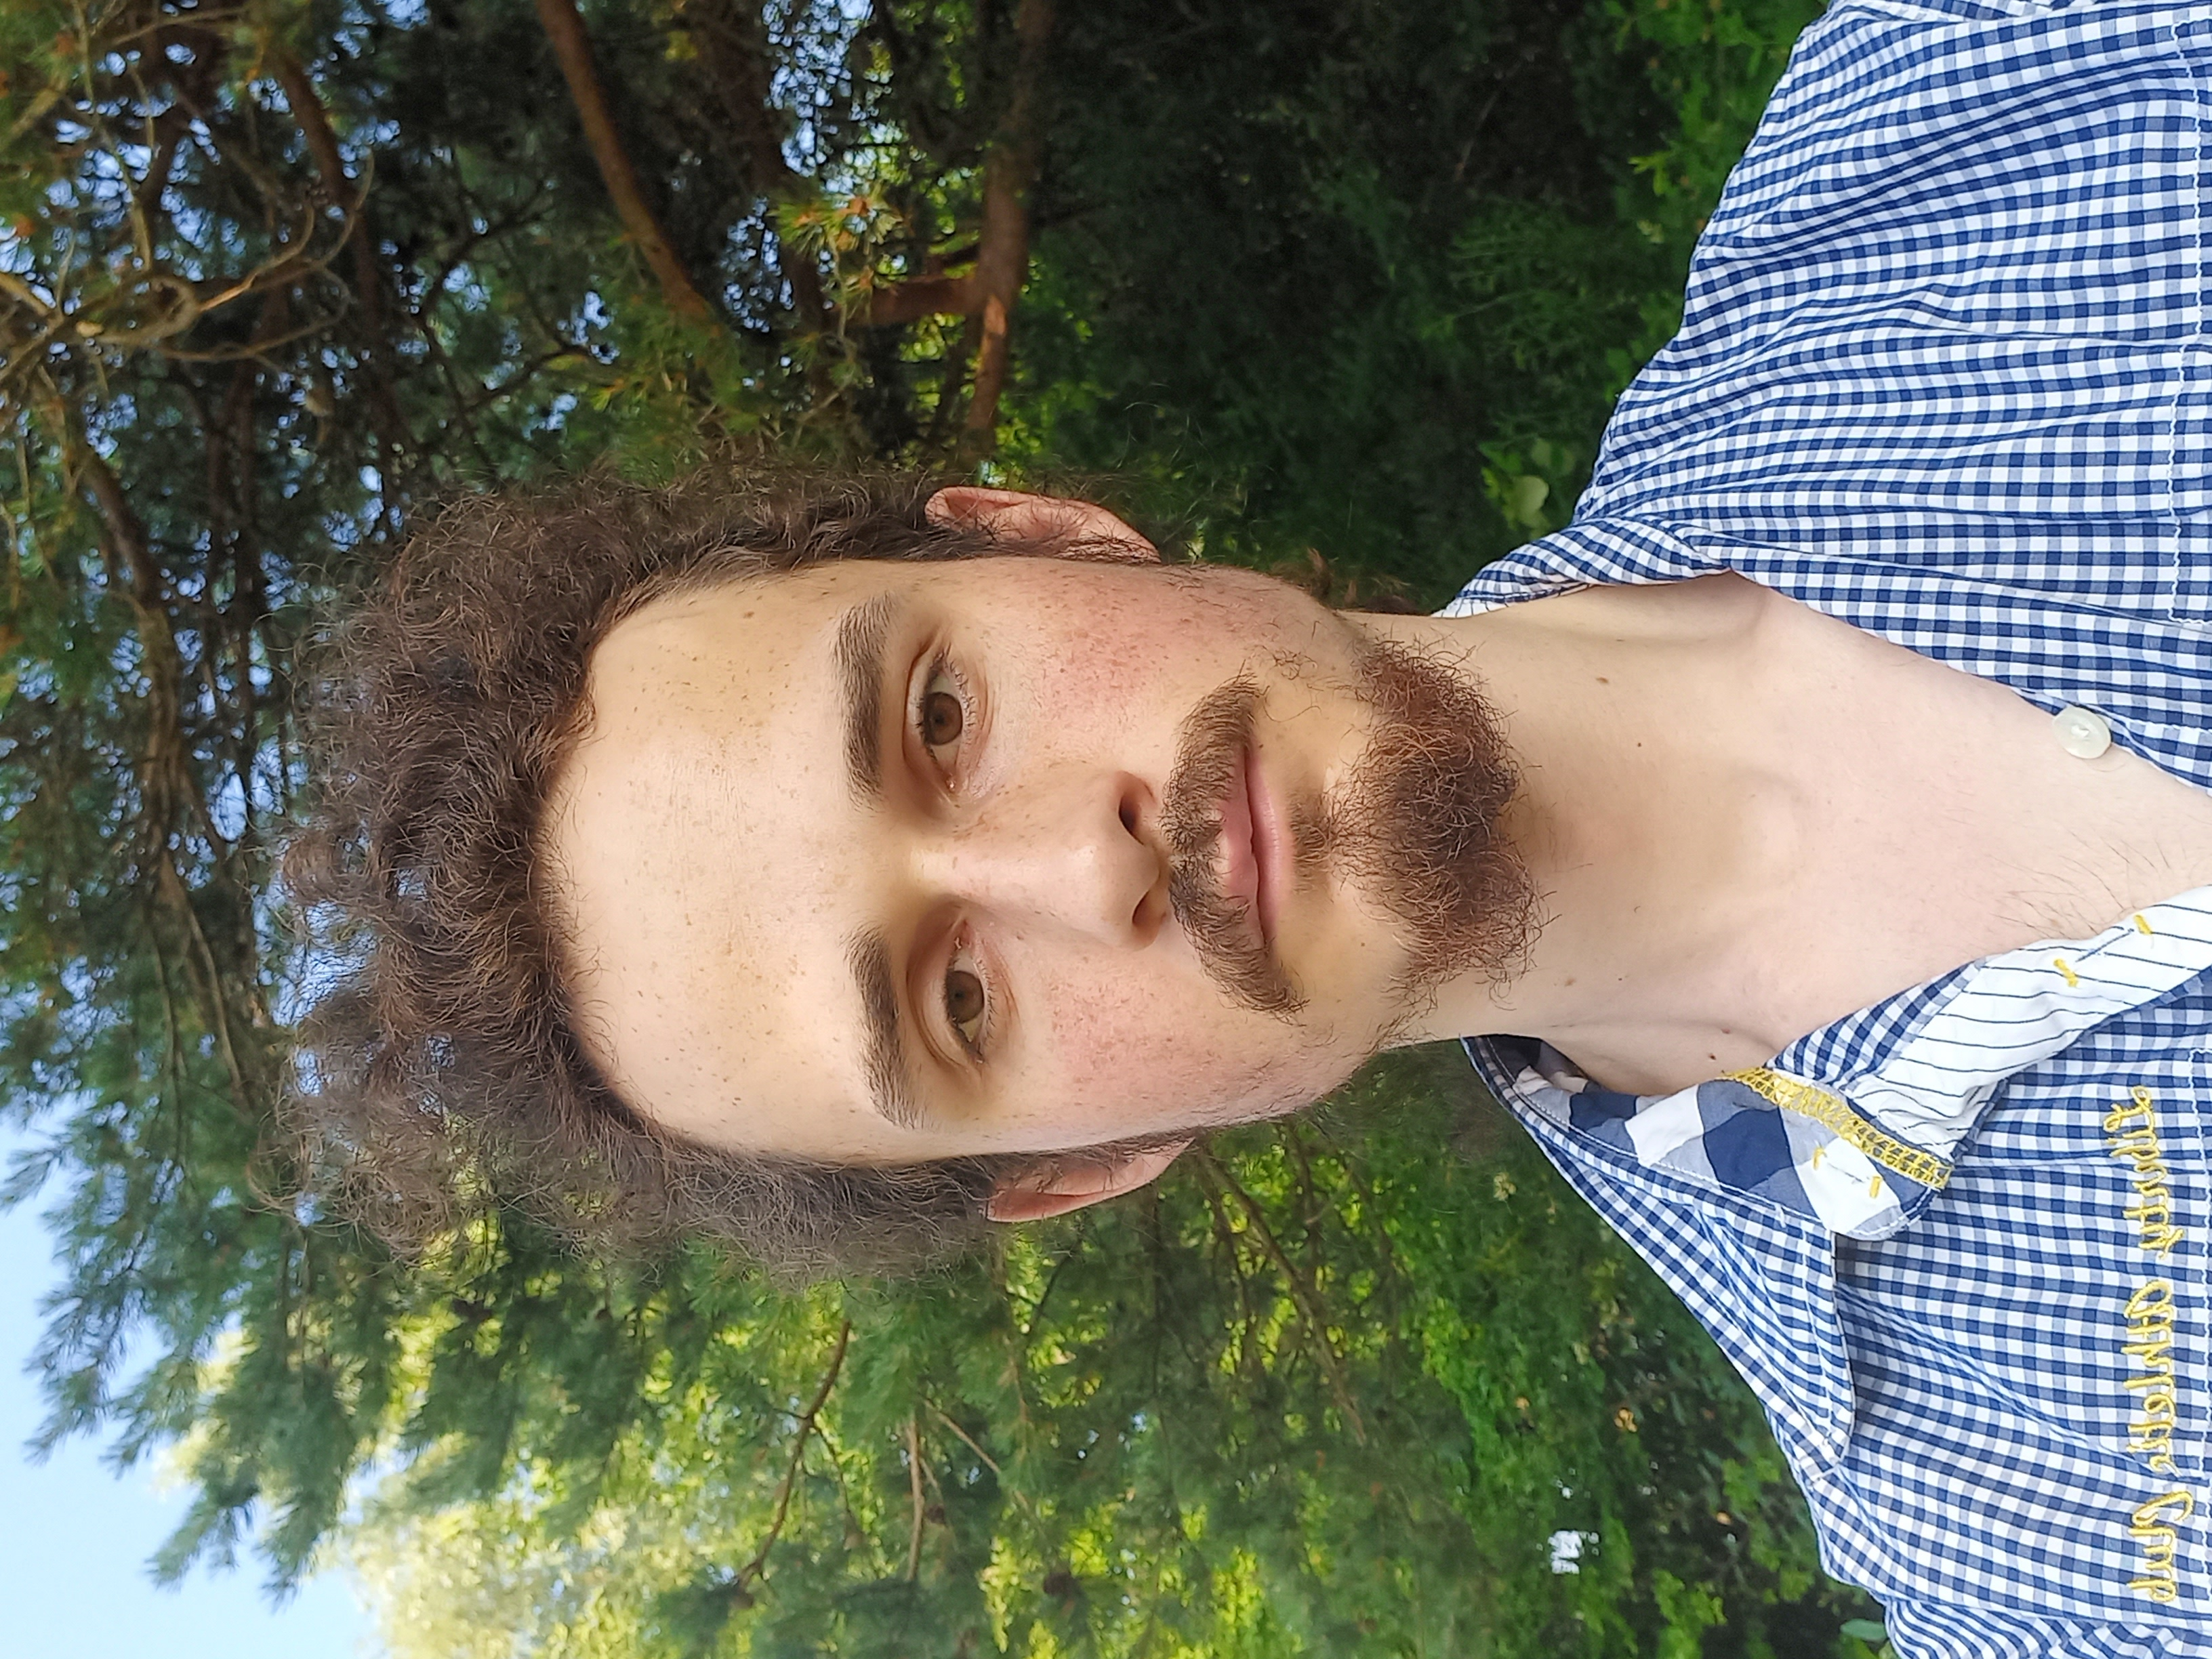
\includegraphics[width=\textwidth, angle=-90]{./img/me.jpg}
		\end{center}
	};
	\node[below = 0pt of picture.south west, anchor = north west, cv text left](contact information){\cvcontact};
	\node[anchor = north west, cv text left](languages) at (contact information.south west){\cvlanguages};
	\node[anchor = north west, cv text left](programming) at (languages.south west){
		\cvprogramming
	};

	%% Draw footer
	\node[below = of education.south west, anchor = north west, cv text right](experience)
	{\small\cvtextmoveout\cvvar{link}};

	%% Finish
	\draw [ultra thick]
		  (split-north) 
	  --  (split-south);
\end{tikzpicture}
\end{document}

